\documentclass[14pt,a4paper,fleqn]{extarticle}
\usepackage[T2A,T1]{fontenc}
\usepackage[utf8]{inputenc}
\usepackage[russian]{babel}
\usepackage{amsmath}
\usepackage{graphicx}
\usepackage{tabularx}
\usepackage{boldline}
\usepackage{makecell}
\usepackage{arydshln}
\usepackage{mathtools}

\graphicspath{ {./images/} }
\setlength{\mathindent}{0pt}
\setlength\parindent{0pt}


\begin{document}
	\begin{titlepage}
		
\includegraphics[scale=0.12]{logo}
		\begin{center}
			\textbf{МИНОБРНАУКИ РОССИИ}\\
			\vspace{0.2cm}
			\textbf{Федеральное государственное бюджетное образовательное учреждение высшего образования}\\
			\textbf{«САНКТ-ПЕТЕРБУРГСКИЙ ГОСУДАРСТВЕННЫЙ ЭКОНОМИЧЕСКИЙ УНИВЕРСИТЕТ»}\\
			\vspace{0.6cm}
			Факультет информатики и прикладной математики\\
			Кафедра прикладной математики и экономико-математических методов\\
			\vspace{1cm}
			\textbf{ОТЧЁТ}\\
			по дисциплине:\\
			\textbf{«Методы оптимизации»}\\
			на тему:\\
			\textbf{«Задание 15. Метод наискорейшего спуска (градиента)»}\\
		\end{center}
		\vspace{1cm}
		Направление: 01.03.02\\
		Обучающийся: Бронников Егор Игоревич\\
		Группа: ПМ-1901\\
		\vfill
		\begin{center}
			Санкт-Петербург\\
			2021\\
		\end{center}
	\end{titlepage}
	\textbf{Дано:}\\
	$f(x_1,x_2,x_3) = (3x_1-3x_2-5)^2 + (6x_1-x_2-x_3-2)^2+(2x_1+5x_2+x_3-1)^2$\\\\
	\textbf{Условие:}\\
	Найти стационарную точку методом наискорейшего спуска (градиента).\\
	
	\textbf{Решение:}\\
	Определим, является ли функция $f(x_1,x_2,x_3)$ выпуклой (вогнутой) или нет.\\
	Найдём первые производные функции:\\
	
	$\dfrac{df}{dx_1} = 98x_1 - 10x_2 - 8x_3 - 58$\\\\
	$\dfrac{df}{dx_2} = -10x_1 + 70x_2 + 12x_3 + 24$\\\\
	$\dfrac{df}{dx_3} = -8x_1 + 12x_2 + 4x_3 + 2$\\
	
	Составим матрицу Гессе $H(X)$ для функции $f(x_1,x_2,x_3)$ и определим знак её угловых миноров:
	\begin{align*}
		H(X) = \begin{pmatrix}
			98 & -10 & -8\\
			-10 & 70 & 12\\
			-8 & 12 & 4\\
		\end{pmatrix}
	\end{align*}
	Вычисляем главные миноры:\\
	$M_1(\boldsymbol{H}) = 98 > 0, \hspace*{0.2cm} M_2(\boldsymbol{H}) = 6760 > 0, \hspace*{0.2cm} M_3(\boldsymbol{H}) = |\boldsymbol{H}| = 10368 > 0$\\
	
	Матрица \textbf{H} -- положительно определённая матрица и, следовательно, $f(x_1, x_2, x_3)$ -- выпуклая функция, которая имеет минимум в некоторой точке $X^*$.\\
	Рассмотрим луч, выходящий из произвольной точки $X = (x_1, x_2, x_3)$, $X^{'} = X + tS$, и направленный в сторону убывания функции $f(x_1, x_2, x_3)$.
	\newpage
	Координаты точек на этом луче имеют следующий вид:\\
	$x_1^{'} = x_1 - t \dfrac{df}{dx_1} = x_1 - t(98x_1 - 10x_2 - 8x_3 - 58)$\\\\
	$x_2^{'} = x_2 - t \dfrac{df}{dx_2} = x_2 - t(-10x_1 + 70x_2 + 12x_3 + 24)$\\\\
	$x_3^{'} = x_3 - t \dfrac{df}{dx_3} = x_3 - t(-8x_1 + 12x_2 + 4x_3 + 2)$\\
	
	Построим вспомогательную функцию $\phi(t)$, равную функции $f(x_1, x_2, x_3)$ на рассматриваемом луче:\\
	
	$\phi(t;X) = f(x_1^{'}, x_2^{'}, x_3^{'}) = f(x_1 - t \dfrac{df}{dx_1}, x_2 - t \dfrac{df}{dx_2}, x_3 - t \dfrac{df}{dx_3}) = $\\\\
	\footnotesize $ = f(x_1 - t(98x_1 - 10x_2 - 8x_3 - 58), x_2 - t(-10x_1 + 70x_2 + 12x_3 + 24), x_3 - t(-8x_1 + 12x_2 + 4x_3 + 2))$\\
	
	\normalsize Градиент $f(x_1,x_2,x_3)$ и вектор $S = -grad\hspace*{0.05cm}f(X)$ определяется выражением:\\
	$grad\hspace*{0.05cm}f(X) = (\dfrac{df}{dx_1}, \dfrac{df}{dx_2}, \dfrac{df}{dx_3}) =$\\\\
	$= (98x_1 - 10x_2 - 8x_3 - 58, -10x_1 + 70x_2 + 12x_3 + 24, -8x_1 + 12x_2 + 4x_3 + 2)$\\
	
	Тогда:\\
	
	$t = \dfrac{grad \hspace*{0.05cm} f(X)\hspace*{0.02cm}grad^T \hspace*{0.05cm} f(X)}{grad \hspace*{0.05cm} f(X)\hspace*{0.02cm}H(X)\hspace*{0.02cm}grad^T \hspace*{0.05cm} f(X)} =$\\
	\scriptsize $ = \dfrac{(98x_1 - 10x_2 - 8x_3 - 58, -10x_1 + 70x_2 + 12x_3 + 24, -8x_1 + 12x_2 + 4x_3 + 2)\begin{pmatrix} 98x_1 - 10x_2 - 8x_3 - 58\\ -10x_1 + 70x_2 + 12x_3 + 24\\ -8x_1 + 12x_2 + 4x_3 + 2\\ \end{pmatrix}}{(98x_1 - 10x_2 - 8x_3 - 58, -10x_1 + 70x_2 + 12x_3 + 24, -8x_1 + 12x_2 + 4x_3 + 2)\begin{pmatrix} 98 & -10 & -8\\ -10 & 70 & 12\\ -8 & 12 & 4\\ \end{pmatrix}\begin{pmatrix} 98x_1 - 10x_2 - 8x_3 - 58\\ -10x_1 + 70x_2 + 12x_3 + 24\\ -8x_1 + 12x_2 + 4x_3 + 2\\ \end{pmatrix}}$\\
	
	\normalsize Выберем в качестве начальной точки точку $X^0 = (x_1^0, x_2^0, x_3^0) = (0,0,0)$, $f(X^0) = 30$.\\
	
	$t_1 = \dfrac{3944}{400856} = 0.0098$
	\newpage
	$x_1^1 = x_1^0 - t_1(98x_1^0 - 10x_2^0 - 8x_3^0 - 58) = 0.570659$\\
	$x_2^1 = x_2^0 - t_1(-10x_1^0 + 70x_2^0 + 12x_3^0 + 24) = -0.236135$\\
	$x_3^1 = x_3^0 - t_1(-8x_1^0 + 12x_2^0 + 4x_3^0 + 2) = -0.0196779$\\
	
	$f(X^1) = 10.5976$\\
	
	На следующей итерации выполняем те же шаги для точки $X^1 = (x_1^1, x_2^1, x_3^1) = (0.570659, -0.236135, -0.0196779)$\\
	
	$t_2 = \dfrac{32.5349}{127.1346} = 0.255909$\\
	
	$x_1^2 = x_1^1 - t_2(98x_1^1 - 10x_2^1 - 8x_3^1 - 58) = 0.4572$\\
	$x_2^2 = x_2^1 - t_2(-10x_1^1 + 70x_2^1 + 12x_3^1 + 24) = -0.627119$\\
	$x_3^2 = x_3^1 - t_2(-8x_1^1 + 12x_2^1 + 4x_3^1 + 2) = 1.38209$\\
	
	$f(X^2) = 6.4346$\\
	
	Создадим функцию в Wolfram Mathematica и при помощи неё проделаем оставшиеся итерации:\\
	
	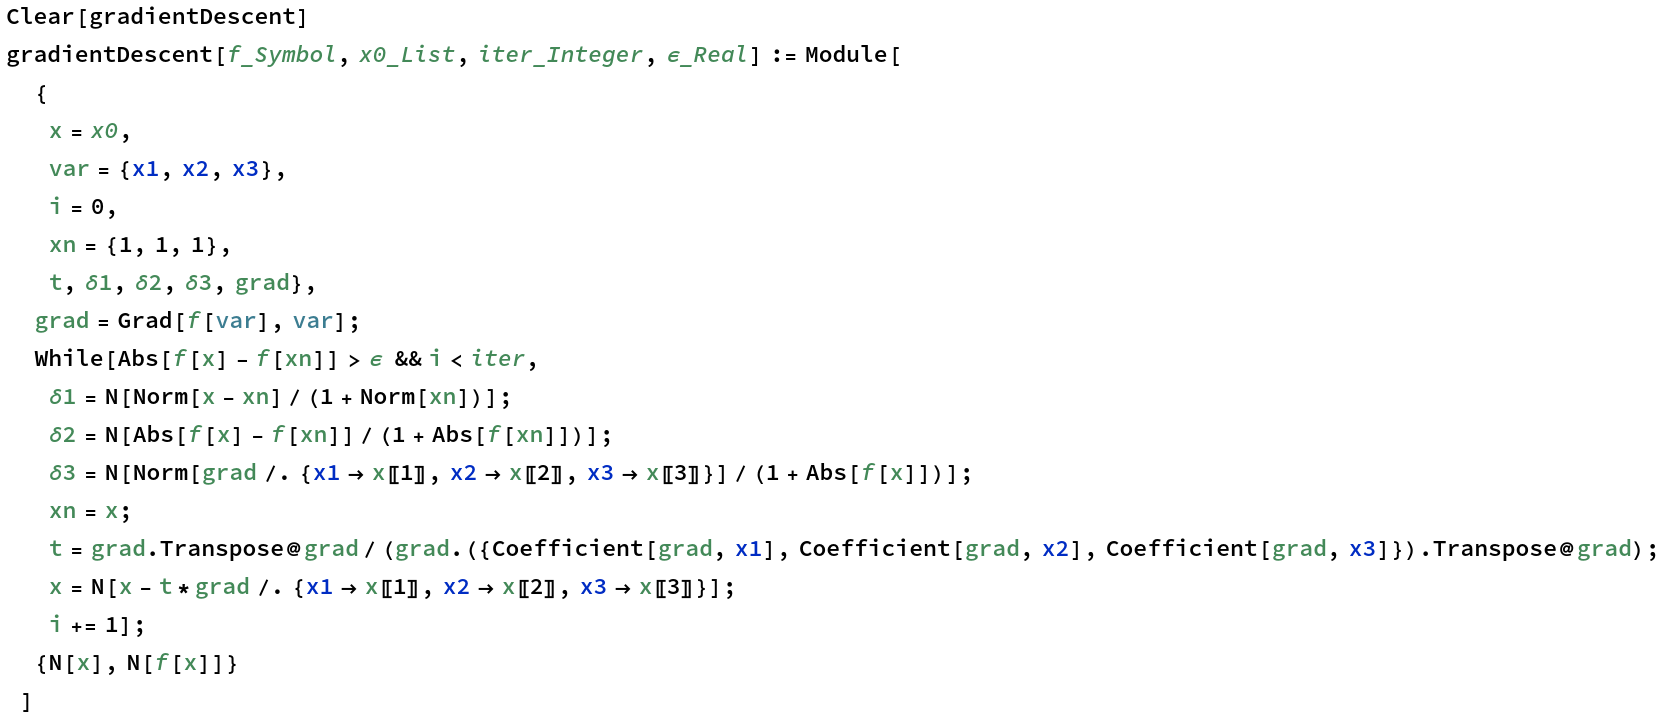
\includegraphics[scale=0.3]{wolfram}
	
	\newpage
	
	Останавливаем итерационный процесс, когда достигли близкого к точному решению ответа.\\
	
	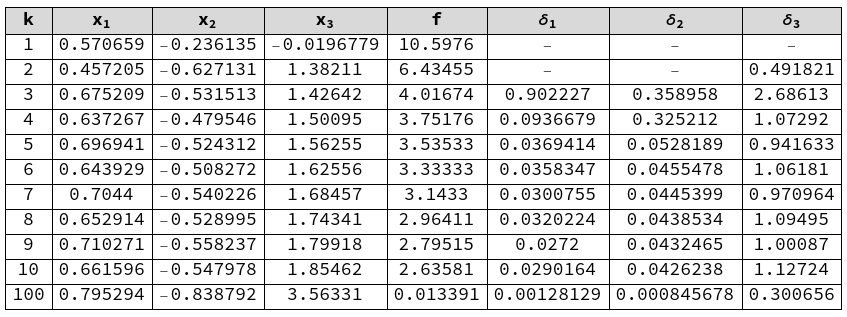
\includegraphics[scale=0.55]{iterations}
	
	Точное значение целевой функции в точке минимума равно:\\
	
	$f(X^*) = f(\dfrac{29}{36}$, $-\dfrac{31}{36}, \dfrac{133}{36}) = 0$\\\\
	$X^* = (\dfrac{29}{36}$, $-\dfrac{31}{36}, \dfrac{133}{36}) \approx (0.805556, -0.861111, 3.69444)$\\
	
	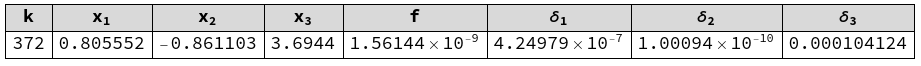
\includegraphics[scale=0.5]{itog}
\end{document}